%lab report 3 of midpoint ellipse drawing algorithm
\documentclass[12pt]{article}

\usepackage{amsmath}
\usepackage{graphicx}
\usepackage[a4paper]{geometry}
\usepackage{times}

\geometry{
  textwidth=\dimexpr\paperwidth-29mm,
  textheight=\dimexpr\paperheight-32mm,
  noheadfoot,
  nomarginpar
}

\setlength{\topskip}{0mm}
\setlength{\parindent}{0mm}

\title{Midpoint Ellipse Drawing Algorithm}
\date{}
\author{}

\begin{document}
	\maketitle
	\vspace{-2cm}

	\section{Objective}
	To draw an ellipse using the midpoint ellipse drawing algorithm.

	\section{Theory}
	
	\subsection{Midpoint Ellipse Drawing Algorithm}
	The midpoint ellipse algorithm is an algorithm used to determine the points needed for drawing an ellipse. It is a variant of Bresenham's circle algorithm where the calculation of \textit{d} is altered to accommodate for the ellipses' eccentricity.
	It makes use of the fact that the sum of the slopes of any point on an ellipse to its foci is always constant. The algorithm exploits this property to determine the next point to plot at each iteration.
	It is similar to the midpoint circle algorithm. The only difference is that the decision parameter is calculated using the midpoint ellipse formula. Since it can be used to draw circles as well as ellipses, it can be said to be a more generalized
	form of the circle drawing algorithm.

	\section{Algorithm}
	\begin{enumerate}
		\item Input the center of the ellipse, radius in x and y direction.
		\item Calculate the initial value of the decision parameter in region 1 as $p_1 = b^2 - a^2b + \frac{1}{4}a^2$.
		\item At each $x_k$ position starting at k = 0, perform the following test:
		\begin{enumerate}
			\item If $p_k < 0$, the next point along the ellipse at $x_{k+1}$ is chosen to be $(x_k + 1, y_k)$ and $p_{k+1} = p_k + 2b^2x_{k+1} + b^2$.
			\item If $p_k \geq 0$, the next point along the ellipse at $x_{k+1}$ is chosen to be $(x_k + 1, y_k - 1)$ and $p_{k+1} = p_k + 2b^2x_{k+1} - 2a^2y_{k+1} + b^2$.
		\end{enumerate}
		\item Repeat step 3 until $2b^2x \geq 2a^2y$.
		\item At each yk position starting at k = 0, perform the following test:
		\begin{enumerate}
			\item If $p_k > 0$, the next point along the ellipse at $y_{k+1}$ is chosen to be $(x_k, y_k - 1)$ and $p_{k+1} = p_k - 2a^2y_{k+1} + a^2$.
			\item If $p_k \leq 0$, the next point along the ellipse at $y_{k+1}$ is chosen to be $(x_k + 1, y_k - 1)$ and $p_{k+1} = p_k + 2b^2x_{k+1} - 2a^2y_{k+1} + a^2$.
		\end{enumerate}
		\item Repeat step 5 until $y_{k+1} = 0$.
	\end{enumerate}

	\newpage
	\section{Source Code}
	\begin{verbatim}
	#include <graphics.h>
	#include <math.h>
	
	void midpointEllipse(int xc, int yc, int a, int b)
	{
	    int x, y, p;
	    x = 0;
	    y = b;
	
	    //initial decision parameter
	    p = b * b - a * a * b + a * a / 4;
	
	    while (2 * x * b * b < 2 * y * a * a)
	    {
	        putpixel(xc + x, yc + y, GREEN);
	        putpixel(xc - x, yc + y, GREEN);
	        putpixel(xc + x, yc - y, GREEN);
	        putpixel(xc - x, yc - y, GREEN);
	        if (p < 0)
	        {
	            x = x + 1;
	            p = p + 2 * b * b * x + b * b;
	        }
	        else
	        {
	            x = x + 1;
	            y = y - 1;
	            p = p + 2 * b * b * x - 2 * a * a * y + b * b;
	        }
	    }
	    p = b * b * (x + 0.5) * (x + 0.5) + a * a * (y - 1) * (y - 1) - a * a * b * b;
	    while (y >= 0)
	    {
	        putpixel(xc + x, yc + y, GREEN);
	        putpixel(xc - x, yc + y, GREEN);
	        putpixel(xc + x, yc - y, GREEN);
	        putpixel(xc - x, yc - y, GREEN);
	        if (p > 0)
	        {
	            y = y - 1;
	            p = p - 2 * a * a * y + a * a;
	        }
	        else
	        {
	            y = y - 1;
	            x = x + 1;
	            p = p + 2 * b * b * x - 2 * a * a * y + a * a;
	        }
	    }
	}

	\end{verbatim}
	\section{Output}

	\begin{figure}[!h]
		\hspace*{-1cm}
		\centering
		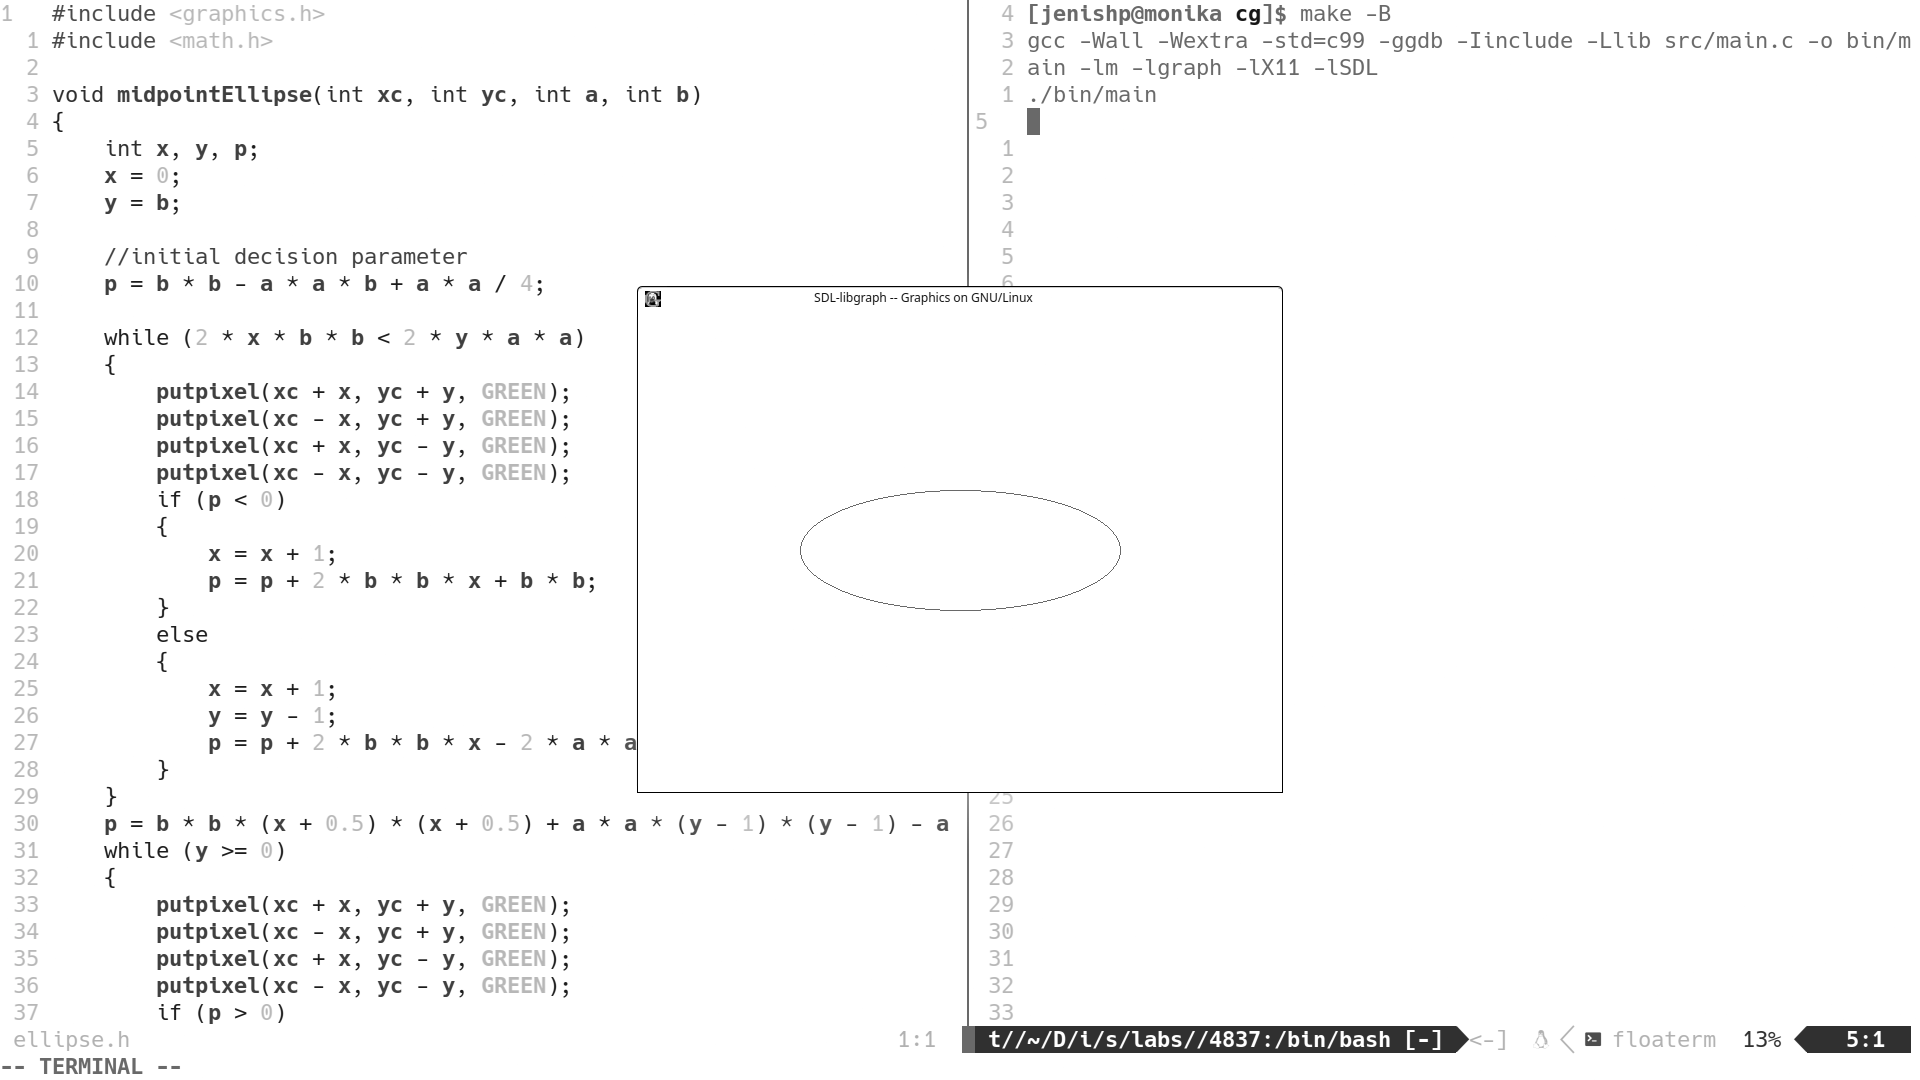
\includegraphics[width=1.01\linewidth]{output3.png}
		\caption{Midpoint Ellipse Drawing Algorithm}
		\label{fig:}
	\end{figure}

	\section{Conclusion}
	We have successfully drawn an ellipse using midpoint ellipse drawing algorithm.
	Ellipses of various eccentricities can be drawn using this algorithm. Drawing of
	circles is a special case of this algorithm and was achieved to demonstrate that
	the algorithm is a generalized version of the midpoint circle drawing algorithm.

\end{document}

